\section{Pianificazione delle attività}
\label{sez:pianificazione-attivita}

Ho effettuato la pianificazione delle attività seguendo un approccio iterativo e collaborativo, con l'obiettivo di garantire una gestione efficace del progetto.\\
Durante la prima settimana, ho lavorato alla definizione delle \gls{user-stories}, che hanno permesso di identificare e organizzare le funzionalità principali del progetto in base alla priorità e al valore per l’utente.\\
Per la lista delle \gls{user-stories} si veda la {\hyperref[subsubsec:epic-stories]{sezione §3.2.1}}.\\

\noindent Successivamente, insieme al \textit{tutor} aziendale, le attività sono state suddivise in \gls{sprint} settimanali.\\
In ogni \gls{sprint} abbiamo selezionato specifiche \gls{user-stories} da completare, tenendo conto delle loro priorità, mantenendo un carico di lavoro sostenibile per il periodo di una settimana. \\
Per ciascun \gls{sprint} ho definito dei criteri di accettazione, ovvero parametri chiari e verificabili che indicano quando un'attività può essere considerata completata. \\
Questi criteri, stabiliti in collaborazione con il \textit{tutor} aziendale, hanno assicurato una qualità elevata del lavoro svolto ed una comprensione condivisa degli obiettivi. \\
Questo approccio mi ha permesso di monitorare costantemente i progressi e garantire un miglioramento continuo durante ogni iterazione del progetto.


\pagebreak
\subsection{Pianificazione settimanale}
\label{sez:pianificazione-settimanale}

\section*{\textit{Sprint} 1: Studio tecnologie (25 Settembre - 1 Ottobre)}
\textbf{Obiettivo:} Studio delle tecnologie fondamentali per il progetto, creazione \gls{user-stories} e della pianificazione.\\  

\noindent \textbf{Descrizione:}\\  
\noindent In questo \gls{sprint}, l'obiettivo principale è acquisire familiarità con le tecnologie che verranno utilizzate nel progetto, come \textit{AWS Bedrock}, \textit{AWS Cognito}, \textit{React}, \textit{NestJS}, \textit{MongoDB}, \textit{Puppeteer} ed altri strumenti correlati.\\
Ho inoltre stilato le \gls{user-stories} e la pianificazione settimanale.\\

\section*{\textit{Sprint} 2: Implementazione autenticazione con \textit{AWS Cognito} (2 Ottobre - 8 Ottobre)}
\textbf{Obiettivo:} Implementare il sistema di autenticazione utilizzando \textit{AWS Cognito}.\\  

\noindent \textbf{Descrizione:}\\  
\noindent Questo \gls{sprint} si concentra sull'implementazione del flusso di \textit{login} per gli utenti utilizzando \textit{AWS Cognito}. \\
Ho sviluppato il sistema di autenticazione e autorizzazione, consentendo agli utenti di accedere e gestire il proprio \textit{account}. \\
Ho inoltre implementato messaggi di errore chiari in caso di credenziali errate.\\

\section*{\textit{Sprint} 3: Visualizzazione, ricerca ed eliminazione dei progetti (9 Ottobre - 15 Ottobre)}
\noindent \textbf{Obiettivo:} Implementare la visualizzazione dei progetti e la loro ricerca.\\

\noindent \textbf{Descrizione:}\\  
\noindent In questo \gls{sprint}, ho sviluppato la funzionalità per visualizzare la lista dei progetti, cercare progetti specifici tramite l’applicazione di filtri e l’eliminazione di un progetto.\\  


\section*{\textit{Sprint} 4: Implementazione \textit{preset} e bozze di progetto (16 Ottobre - 22 Ottobre)}
\textbf{Obiettivo:} Implementare la pagina di creazione dei progetti, da cui è possibile compilare i \textit{preset} o salvarli come bozza.\\

\noindent \textbf{Descrizione:}\\
\noindent In questo \textit{sprint}, ho sviluppato la pagina per la compilazione dei \textit{preset}, da cui è inoltre possibile salvare una bozza compilata (in parte) per essere utilizzata in un secondo momento.\\
Ho inoltre sviluppato la pagina che contiene le informazioni di un singolo progetto, come nome, data di creazione e tutti i capitoli che lo compongono.\\  

\section*{\textit{Sprint} 5: Generazione progetti e \textit{download} PDF (23 Ottobre - 29 Ottobre)}
\textbf{Obiettivo:} Implementare la generazione di progetti ed il \textit{download} dei documenti in formato PDF.\\

\noindent \textbf{Descrizione:}\\
\noindent Questo \textit{sprint} si concentra sulla generazione dei progetti utilizzando i \textit{preset} e sulla possibilità di scaricare il progetto finale in formato PDF.\\
L'utente può scaricare il documento completo per l'archiviazione e/o la condivisione.\\

\section*{\textit{Sprint} 6: Rigenerazione progetti e capitoli (30 Ottobre - 5 Novembre)}
\textbf{Obiettivo:} Implementare la rigenerazione dei progetti e la possibilità di rigenerare capitoli specifici.\\

\noindent \textbf{Descrizione:}\\
\noindent In questo \textit{sprint}, ho implementato la funzionalità per rigenerare un progetto completo o singoli capitoli, consentendo all'utente di modificare e aggiornare solo le parti necessarie del progetto, mantenendo intatti gli altri capitoli.\\

\section*{\textit{Sprint} 7: Gestione della versione e rifiniture finali (6 Novembre - 12 Novembre)}
\textbf{Obiettivo:} Gestire la versione dei progetti ed effettuare le rifiniture finali prima dell'attività di \textit{testing}.\\

\noindent \textbf{Descrizione:}\\
\noindent In questo \textit{sprint}, ho sviluppato la funzionalità per gestire la versione dei progetti, permettendo agli utenti di visualizzare, confrontare e ripristinare versioni precedenti.\\
Inoltre, ho completato le ultime rifiniture del sistema, inclusi eventuali miglioramenti all'interfaccia o risoluzioni di \textit{bug}.\\
\pagebreak
\section*{\textit{Sprint} 8: \textit{Testing} e \textit{deployment} (13 Novembre - 19 Novembre)}
\textbf{Obiettivo:} Eseguire i \textit{test} finali, risolvere i \textit{bug} ed effettuare il \textit{deploy} del sistema in produzione.\\

\noindent \textbf{Descrizione:}\\
\noindent Questo \textit{sprint} si concentra sull'attività finale di \textit{testing} del sistema.\\
Ho eseguito i \textit{test} unitari, di integrazione e di performance. Una volta superati i \textit{test}, il sistema sarà pronto per il rilascio in produzione. \\
Ho inoltre creato gli \textit{Swagger} (\textit{OpenAPI}) di tutte le \gls{api}.\\

\noindent La {\hyperref[fig:gantt-chart]{Figura 3.1}} riporta il diagramma di \textit{Gantt} che rappresenta la pianificazione delle attività svolte durante il periodo di stage, suddivise per \gls{sprint} settimanali.\\

\begin{figure}[H]
    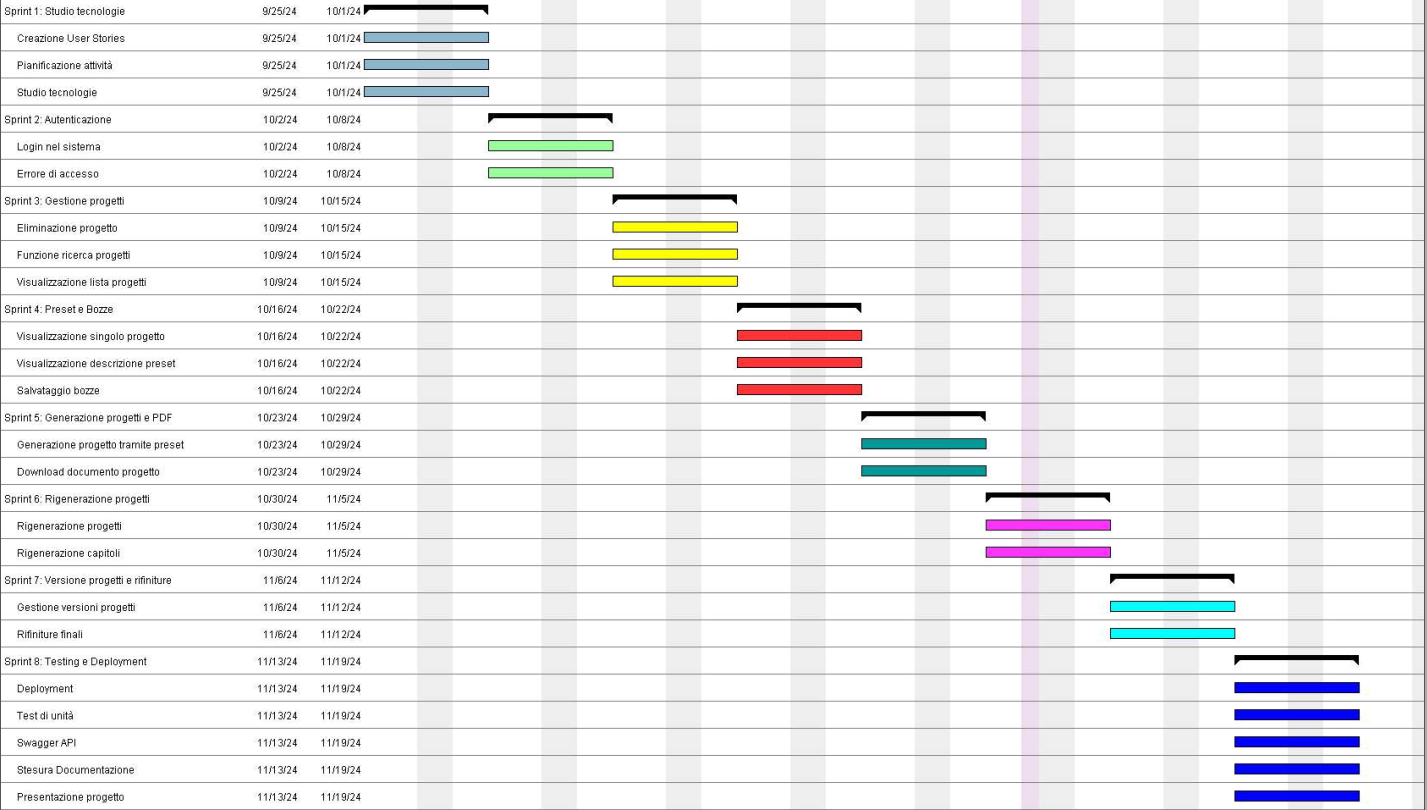
\includegraphics[scale=0.4]{pianificazione/gantt-chart.png}
    \caption{Diagramma di \textit{Gantt} delle attività svolte durante il periodo di stage}
    \label{fig:gantt-chart}
\end{figure}